%!TEX root = ../../../adrien_gomar_phd.tex

\begin{figure}[htp]
  \centering
  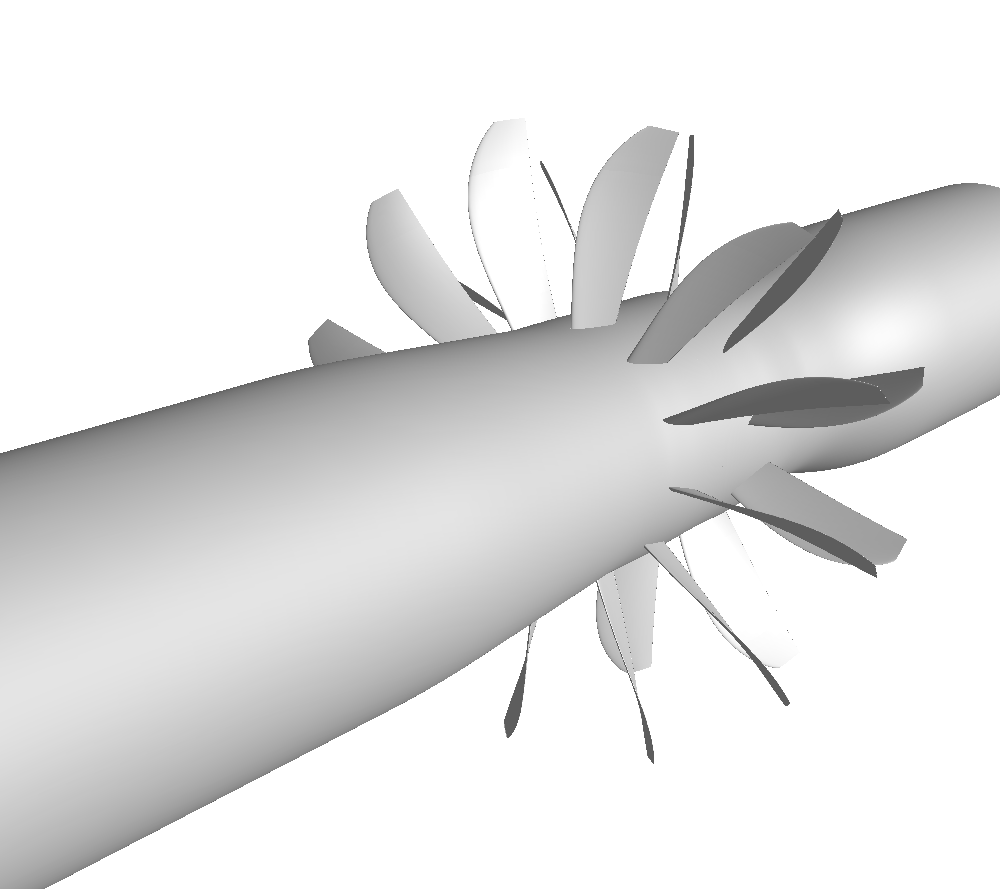
\includegraphics[width=.3\textwidth]{DREAM_HS_wall.png}
  \caption{High-speed isolated contra-rotating open rotor geometry.}
  \label{fig:dream_hs_wall}
\end{figure}

The configuration studied in this Chapter is the same as the
previous one but with a different angle of attack of
the blades as the inflow Mach number is larger. 
The geometry is shown in Figure~\ref{fig:dream_hs_wall}.
This geometry is the High-Speed (HS) version of the previous one, 
representative of the cruise flight condition. The rotation speed is kept
almost constant between the two configurations, meaning that
the only way to ensure
a proper adaptation of the velocity field is to change the angle of 
attack of the blades.

The main input parameters of the case are recalled in
Tab.~\ref{tab:dream_hs_flight_condition}.
\begin{table}[htp]
  \ra{1.3} \centering
  \begin{tabular}{cccc}
    \toprule
    $M_0$ & $J$ & $M_{tip}$ \\
    \midrule
    $0.73$ & 3.7 & 0.96  \\
    \bottomrule
  \end{tabular}
  \caption{High-speed isolated contra-rotating open rotor flight condition parameters.}
  \label{tab:dream_hs_flight_condition}
\end{table} 
The inflow Mach number is within the transonic range. Its high value
can suggest the appearance of shocks in the flow field. 
This is emphasized by the $M_{tip}$ which is
near from being supersonic.

The same two structural modes are considered for the aeroelastic study of this 
configuration: the second bending/flection mode (2F) and the first torsion mode (1T)
of the front rotor. These were inputs of the current work.

The frequency, mass and stiffness of the modes 
are given with the corresponding modes.
The ratio of the frequency of the blade passing 
frequency of the opposite row, namely the rear rotor,
over the aeroelastic frequency of
each mode varies between 
$3.35 \leq f_{BPF} / f_{AEL} \leq 4.11$. Again,
this last frequency governs the unsteady rigid-motion flow physics 
and will have to be computed alongside with the aeroleastic frequency.
Therefore, the multi-frequential formulation of the
harmonic balance approach will be used to simulate the
aeroelastic response of the blades (see Sec.~\ref{sec:dream_hs_ael_results}).
